%META {"question":"Tam giác ABC vuông tại A. Đoạn thẳng AB là gì của tam giác ABC?","options":["Đường cao ứng với cạnh AC","Trung tuyến ứng với cạnh BC","Tia phân giác của góc B","Cạnh huyền của tam giác"],"answer":0,"note":"AB vuông góc với AC tại A nên AB chính là đường cao hạ từ B xuống cạnh AC. Trong tam giác vuông, hai cạnh góc vuông đóng vai trò là đường cao của nhau."}
\documentclass[border=5pt]{standalone}
\usepackage{tkz-euclide}
% Màu dùng chung cho toàn bộ hình vẽ (ảnh stack với nền tối của web)
\definecolor{tminc}{RGB}{226,232,240}   % chữ + nét chính
\definecolor{tmblue}{RGB}{0,210,255}    % nhấn neon xanh
\definecolor{tmpink}{RGB}{255,0,200}    % nhấn neon hồng
\definecolor{tmgreen}{RGB}{0,255,136}   % nhấn neon xanh lá
\color{tminc}

\begin{document}
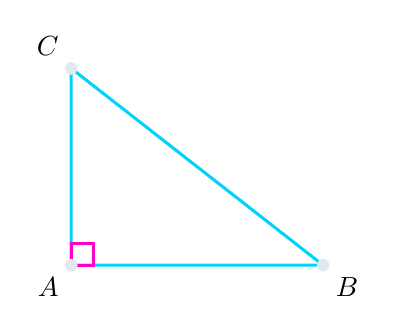
\begin{tikzpicture}[line width=1.1pt]
  \coordinate (A) at (0,0);
  \coordinate (B) at (3.2,0);
  \coordinate (C) at (0,2.5);
  \tkzDrawPolygon[tmblue,line width=1.1pt](A,B,C)
  \tkzMarkRightAngles[size=0.28,color=tmpink,line width=1pt](B,A,C)
  \tkzDrawPoints[size=3.5,color=tminc,fill=tminc](A,B,C)
  \tkzLabelPoint[below left=1pt](A){$A$}
  \tkzLabelPoint[below right=1pt](B){$B$}
  \tkzLabelPoint[above left=1pt](C){$C$}
\end{tikzpicture}
\end{document}
